\documentclass[11pt]{article}
\usepackage{amsmath}
\usepackage{graphicx}
\usepackage{caption}
\usepackage{amssymb}
\usepackage{verbatim}
\usepackage{hyperref}
\usepackage{listings}
\usepackage{float}
\usepackage[thinc]{esdiff}
\usepackage{euscript}
\usepackage{subcaption}
\usepackage{commath}
\setlength{\parindent}{0em}
\newcommand*{\field}[1]{\mathbb{#1}}%
\usepackage{amsthm}
\newtheorem{claim}{Claim}
\captionsetup{labelformat=empty}

\begin{document}
\begin{titlepage} % Suppresses displaying the page number on the title page and the subsequent page counts as page 1
	
	\center % Centre everything on the page
	
	\vspace*{3cm}

	\textsc{Mathematical Tripos, Part 1B}\\
	\textsc{Computational project}
	\begin{center}
      {\huge\bfseries Collapse of a Spherical Cavitation Bubble\\[0.4cm]
}     \end{center}
	 % Title of your document
	
	\vfill
	\vfill\vfill
	
	\includegraphics*[width = 2.675cm, height = 3.1cm]{coat.png}
	\vfill
	\textsc{University of Cambridge}
	%------------------------------------------------
	%	Date
	%------------------------------------------------
	\vspace*{\fill}
	\vfill\vfill
	{\large\today} 
	\vfill
	% Push the date up 1/4 of the remaining page	
\end{titlepage}

\section{Introduction}
For a spherical bubble of radius $R(t)$, its radius changes at rate $\dot{R(t)}$ while remaining spherical, so it has boundary condition $$\mathbf{u\cdot n}= \dot{R(t)}\mathbf{e_{r} \cdot n}$$ Assume that the fluid starts from rest and there is incompressible, from knowledge in fluid dynamics the surrounding flow is identically a mass source if $\dot{R(t)}>0$ , or a sink source otherwise.
Then the scalar potential and the velocity field are given by $$ \phi =-\frac{R^2\dot{R}}{r};\ \ \mathbf{u} = \nabla\mathbf{\phi} = \frac{R^2\dot{R}}{r^{2}}\mathbf{e_{r}}$$
Then by time independent Bernoulli, the quantity
$$ \tilde{H(t)} = \frac{\partial\phi}{\partial t} + \frac{1}{2}\abs{\mathbf{u}}^2 +\frac{p}{\rho}$$ is invariant in space.
Therefore we have the following equations:$$\frac{\partial}{\partial t}\left(-\frac{R^2\dot{R}}{r}\right)+\frac{R^4 \dot{R}^2}{2r^4}+\frac{p(r,t)}{\rho} = \frac{p(\infty,t)}{\rho}$$
after scaling we have $\rho=1,\ R(0)=1,\ p(\infty, t)=1$, rearranging to obtain \begin{equation}
p(r,t) =1+\frac{1}{r}\frac{d}{dt}\left({R^2\frac{dR}{dt}}\right)-\frac{R^4}{2r^4} \left(\frac{dR}{dt}\right)^2 \tag{1.1}
\end{equation}
\section{Analytic solutions}
\subsection{Question 1}
Substitute the boundary condition given by $$p(R,t) = -\frac{2\lambda}{R}$$, we have 
$$R\ddot{R}+\frac{3}{2}\dot{R}^2 = -1-\frac{2\lambda}{R}$$,
with integrating factor $R^2\dot{R}$ $$\frac{1}{2}\frac{d}{dt}(R^3\dot{R}^2) = -\dot{R}R^2-2\lambda\dot{R}R$$
Then we integrate to have the following:
$$\frac{1}{2} R^3\dot{R}^2 = -\frac{R^3}{3} - \lambda R^2 + const.$$ Finally,  we impose the initial condition $R(0) = 1;\ \dot{R(0)} = 0$, $const = \lambda +\frac{1}{3}$, and 
\begin{equation}
\dot{R}^2 = \frac{2}{3} \left(\frac{1}{R^3}-1\right)+2\lambda\left(\frac{1}{R^3}-\frac{1}{R}\right) \tag{2.1.1}
\end{equation}
From this equation, under $\lambda>0$, we can see that  $\dot{R}$ is negative as  $R\leqslant1$ from $RHS\geqslant0$
The plot follows.
\begin{figure}[H]
\centering
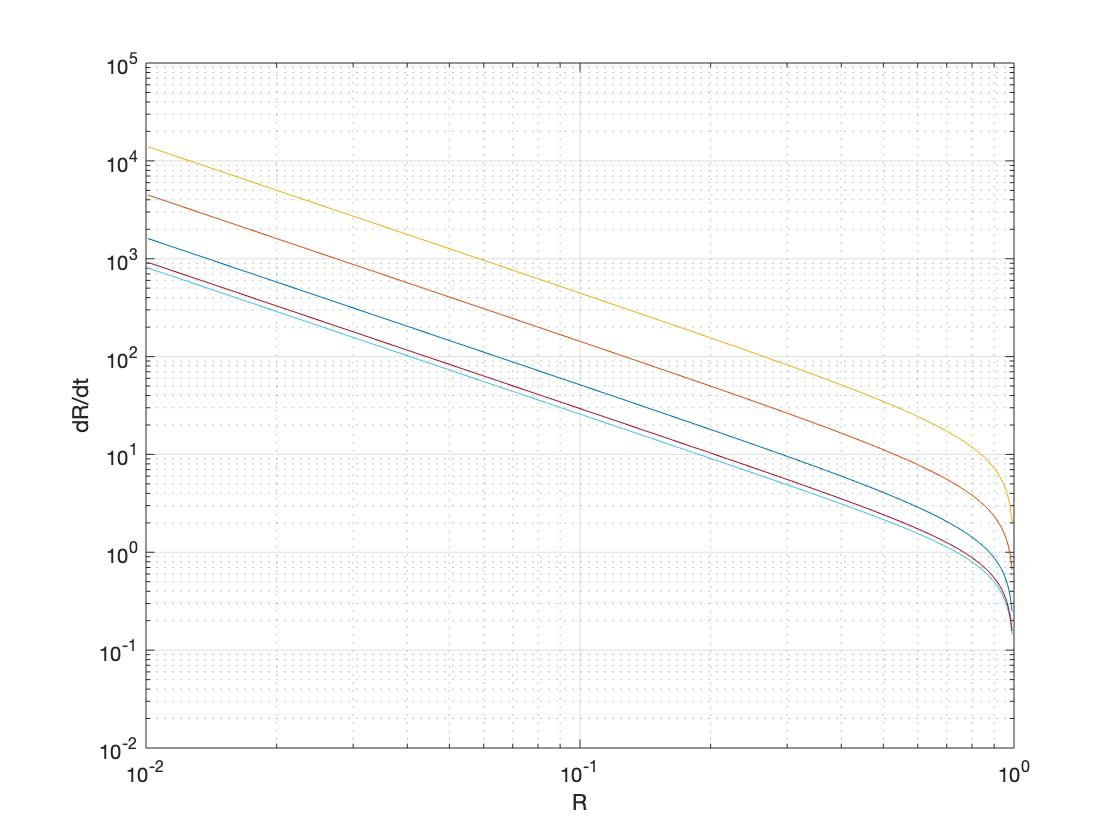
\includegraphics[width = 12cm, height = 9cm]{Q1.jpg}
\caption{Figure 1.1: Plot of $\abs{\dot{R}}$ against $R$ for $\lambda=0.0,\ 0.1,\ 1.0,\ 10.0\ and\ 100.0$ (from below to above) in log scale }
\end{figure}
Comments: When the collapse starts, the speed of contraction increases rapidly, then keeps the trend almost linearly against R as it decreases further from 1. The explanation is that from the differential equation,  $\dot{R}\sim (\frac{2}{3}+2\lambda)R^{-3}$ when $R<<1$, and the non-cubic terms of $R^{-1}$ matter when the contraction starts. It is not accurate when R is extremely small, as the velocity tends to infinity which is impossible.

\subsection{Question 2}
Recall from (1.1) and differentiate(2.1.1), we have the following:
\begin{align*}
p(r,t) &=1+\frac{1}{r}\left(2R\dot{R}^2 + R^2\ddot{R}\right)-\frac{R^4\dot{R}^2}{2r^4} \tag{1.1}\\
\ddot{R}& = \frac{\lambda}{R^2}-(1+3\lambda)\frac{1}{R^4}\ .
\end{align*}
Substitute
\begin{align*}
\alpha = \frac{1}{4}\left(1-4R^3\right)+\frac{3}{4}\lambda\left(1-3R^2\right)\ \ and\ \ \beta = 1-R^3+3\lambda\left(1-R^2\right)\ ,
\end{align*} 
we have
\begin{equation*}       
p(r,R) = 1-\frac{R\beta}{3r^4}+\frac{4\alpha}{3rR^2}\ . \tag{2.2.1}
\end{equation*}
At time t, R(t) is fixed. Differentiate (2.2.1) with respect to r, 
$$\frac{4R\beta}{3r^5}-\frac{4\alpha}{3r^2 R^2}=0\Rightarrow\ r_{0} = R\sqrt[3]{\frac{\beta}{\alpha}}$$
From 2.1 we learnt that $R\leqslant 1$, so $\beta \geqslant 0$. 
The absolute value of  $r_{0}$ is greater than r if $\beta>\abs{\alpha}$, which is true by the expressions of $\alpha$ and $\beta$.\newline
Observe that $p \to 1$ as $t \to \infty$, and 
if $\alpha > 0$, the maximum is obtained at $r_{0}$; otherwise p is monotonic in r, and as $p(R,R)<1$ it is increasing. Hence, the maximum is just 1. i.e.
\[p_{max} = 
\begin{cases}
\ 1,     & \alpha<0\\
\ 1+R^{-3}\left(\alpha^4/\beta\right)^{1/3}, & \alpha>0
\end{cases}\]
The plot follows.
\begin{figure}[H]
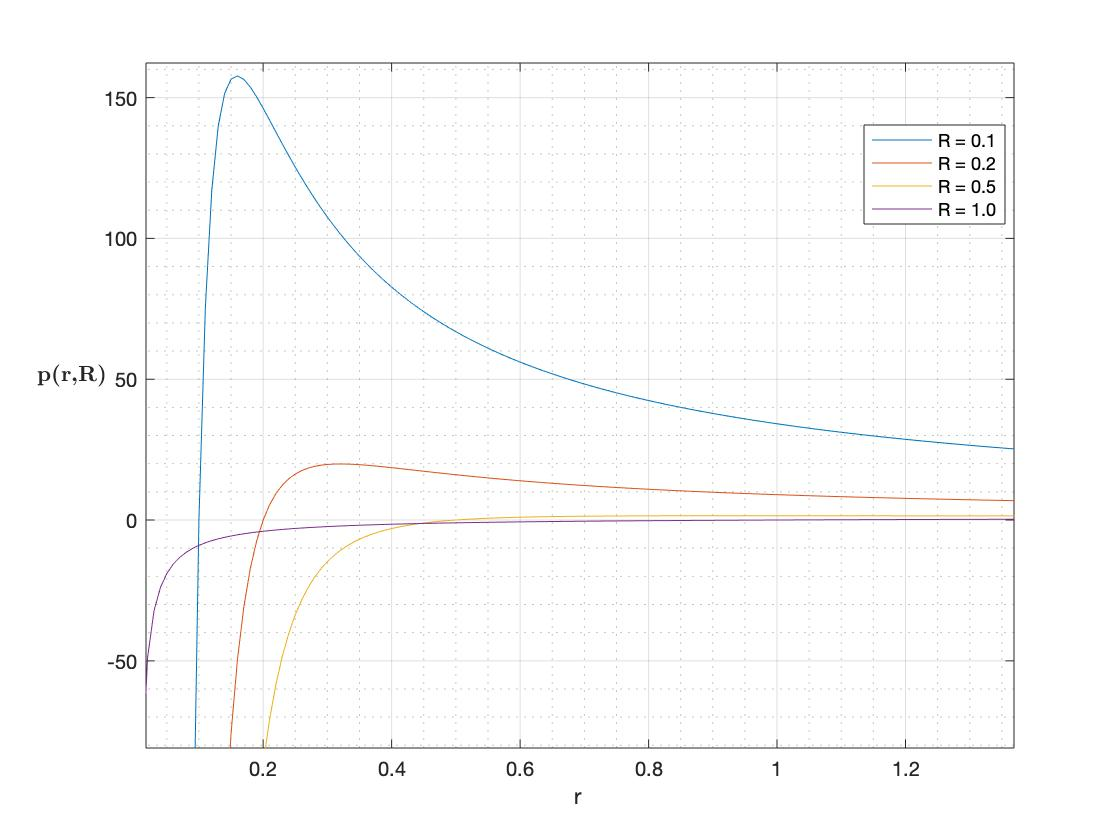
\includegraphics[width = 12cm, height = 9cm]{Q2.jpg}
\caption{Figure 2.1: Plot of p(r,R) against r for $ \lambda = 0$}
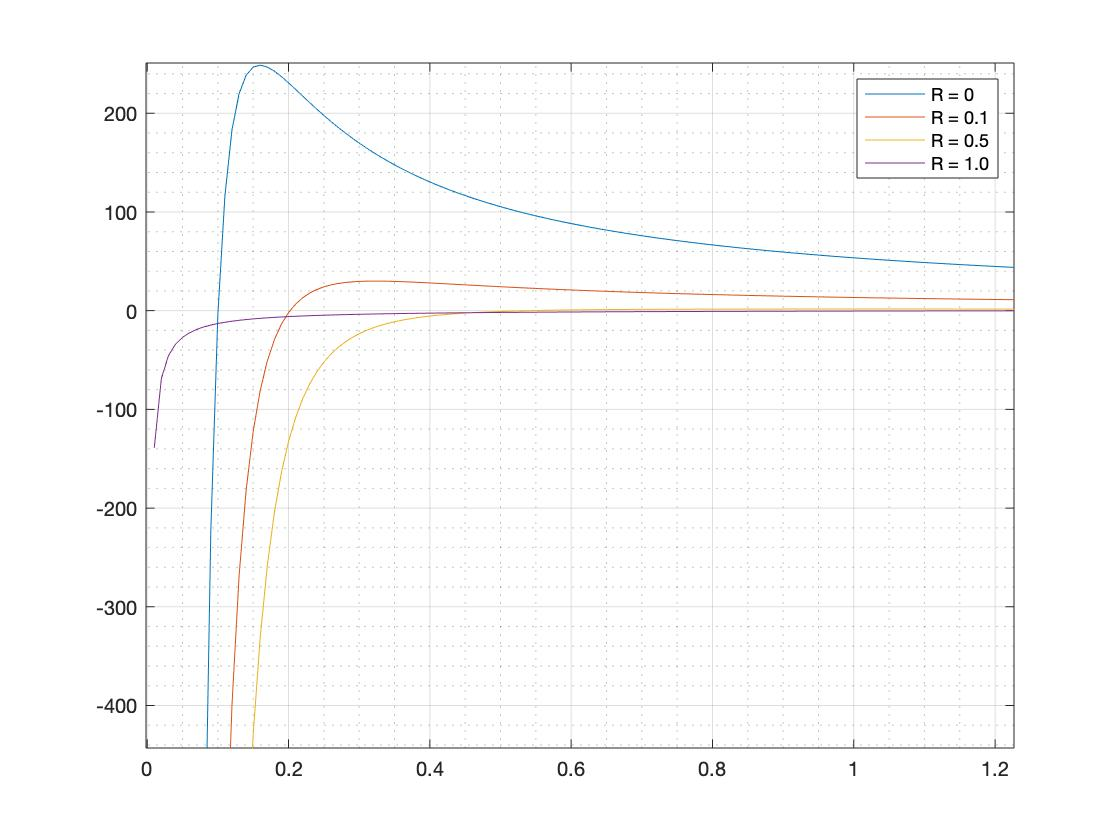
\includegraphics[width = 12cm, height = 9cm]{Q2(2).jpg}
\caption{Figure 2.2: Plot of p(r,R) against r for $\lambda = 0.2$}
\end{figure}
\begin{figure}[H]
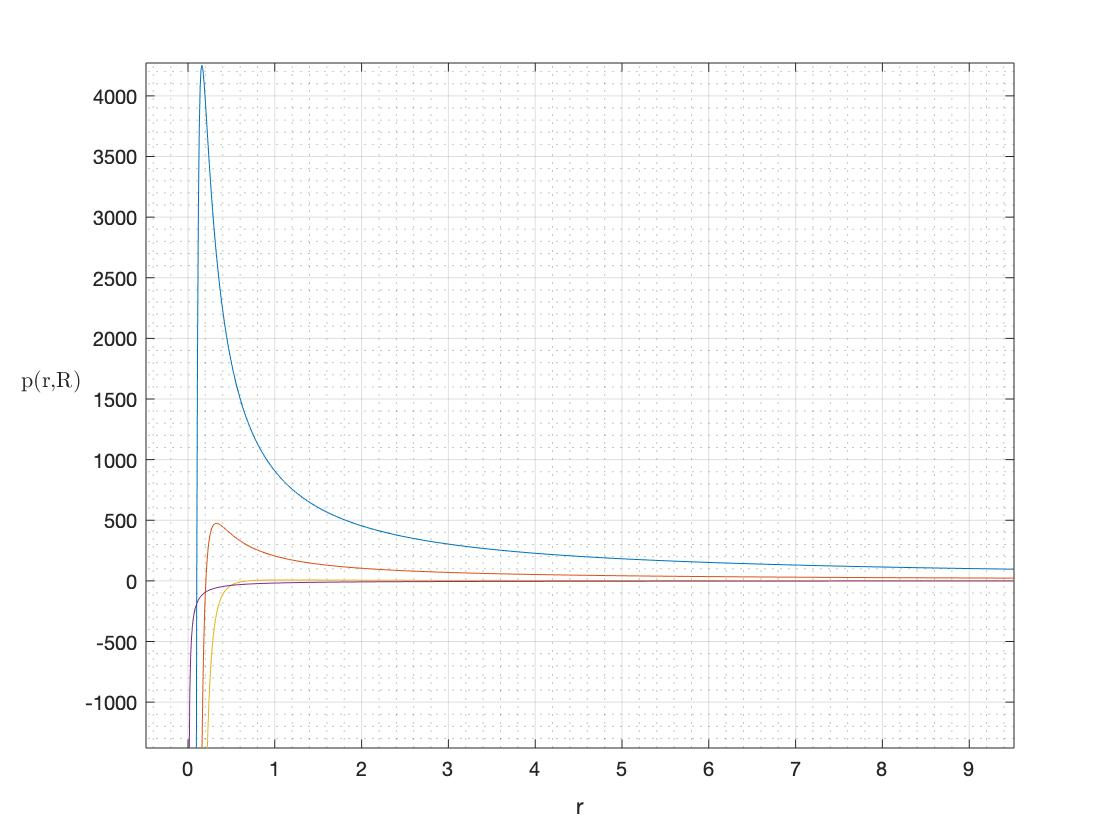
\includegraphics[width = 12cm, height = 9cm]{Q2(3).jpg}
\caption{Figure 2.3: Plot of p(r,R) against r for $\lambda = 9.0$}
\end{figure}
Comments: At time t, the graphs show that when 
$ \alpha > 0$, the largest pressure increases with the surface tension $ \lambda $. Under the same surface tension, suppose $R_{1}>R_{2}$, then at a certain value of $r \geqslant \sup\lbrace{R_{1}, R_{2}\rbrace}$ the pressure obeys $p_{1}<p_{2}$. i.e. as the bubble contracts, the pressure at a fixed point away from the surface of bubble at a certain distance decreases.
\section{No surface tension case}
\subsection{Question 3}
Define $x = R^{5/2}$, take its time derivative, we have: $\dot{x} = \frac{5}{2}\dot{R}R^{\frac{3}{2}}$ 
substitute this into (2.1.1) we have the following:
$$\dot{x}^2 = \frac{25}{6}(1-x^{\frac{6}{5}})+\frac{25}{2}\lambda(1-x^{\frac{4}{5}})$$
We choose the negative root here, so: 
\begin{equation*}
\dot{x} = -\frac{5}{2}\left[\frac{2}{3}\left(1-x^{\frac{6}{5}}\right)+2\lambda\left(1-x^{\frac{4}{5}}\right)\right]^{1/2} \tag{3.1.1}
\end{equation*}
With $x=1\ at\ t=0$.
The justification of choosing the negative root is that previously we have seen $R\leqslant 1$ as square is non-negative, then dR/dt must be negative as the radius can only decrease. \newline\newline
From a physical point of view, the bubble is a cavity, so the pressure inside the bubble (which is 0) is much smaller than that from the fluid surrounding the bubble, hence the bubble contracts due to the pressure difference.\newline\newline
All previous discussion has based on the fact that the surface pressure is $-2\lambda/R$ in a bubble cavitation case. If $p(R,t) = p_{0} - 2\lambda/R$ for some value $p_{0}$ induced by interior pressure of the bubble, or when $\lambda < 0$ in the cavity case. Then it is possible to have $\dot{x}>0$ , R increases before it decreases, so the bubble expands before it contracts.
\newline\newline
The usual benefit of a high order method is that when the step size$h \to 0 $, it converges faster to the exact solution. The local truncation error is of the form $\frac{d^{k}x}{dt^{k}}h^m$. When $x\to 0$, $\frac{d^{k}x}{dt^{k}} \to 0$ for all k as well, so the local truncation error is already subtle and the advantage is thus much less evident as $h \to 0$.
\newline\newline
To avoid convergence to $x=1$, we can do the following: Set $x = 1-\eta$, where $\eta(0) = 0$
Then (3.1.1) becomes $$\dot{\eta} = \frac{5}{2}[\frac{2}{3}(1-(1-\eta)^{\frac{6}{5}})]^{\frac{1}{2}}$$
For small t, $(1-\eta)^{\frac{6}{5}} \approx 1-\frac{6}{5}\eta$, then we have$\dot{\eta} = \sqrt{5}\eta^{\frac{1}{2}}$ Hence $\eta = \frac{5}{4}t^{2} $
So we have $x \approx 1-\frac{5}{4}t^{2}$. We choose $t_{0} = 0.0001$ to be the starting time, then we have the following figure:
\begin{figure}[H]
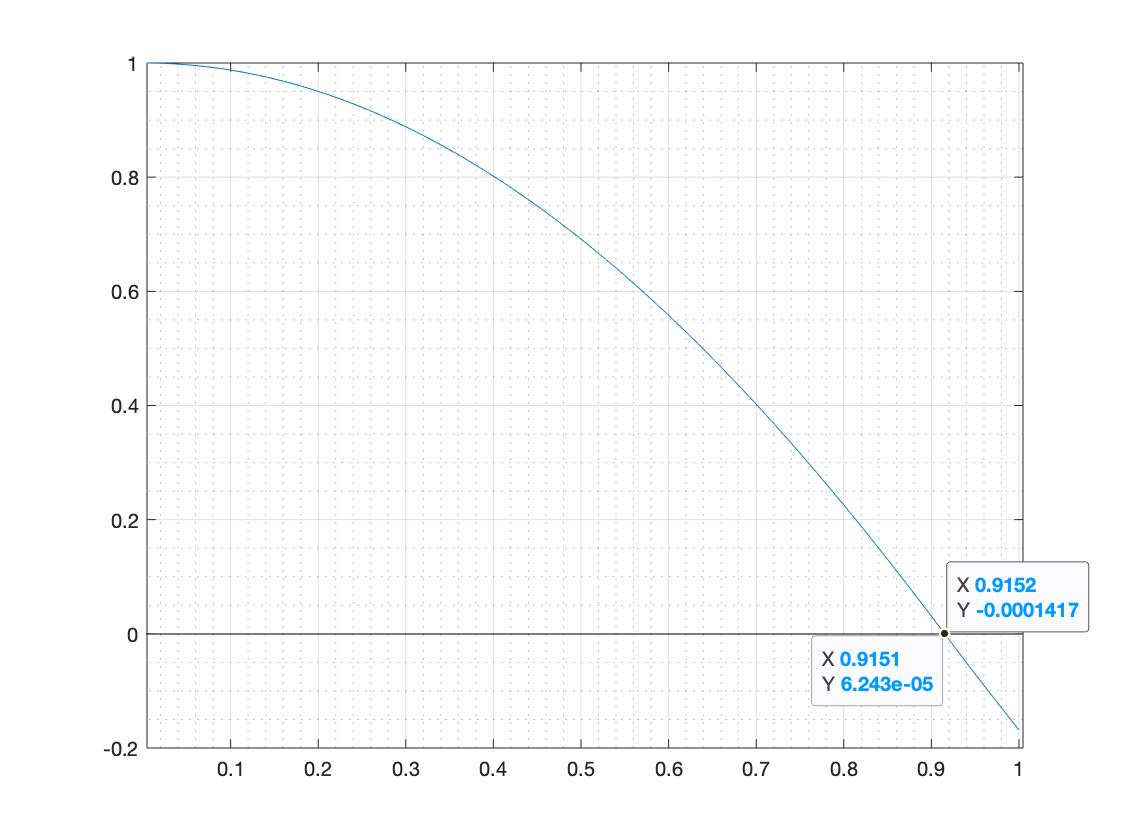
\includegraphics[width = 12cm, height = 9cm]{Q3.jpg}
\caption{Figure 3.1.1: Numerical solution of x}
\end{figure}

Make substitution $x = sin^{5/3}\theta$, we have the following $$\frac{5}{3}\sin^{2/3}\theta \cos\theta \dot{\theta} = -\frac{5}{2}\sqrt{\frac{2}{3}}\cos\theta $$ i.e.
$$\dot{\theta} = -\sqrt{\frac{3}{2}}sin^{-2/3}\theta$$
$$t_{c} = \sqrt{\frac{2}{3}}\int_{0}^{\frac{\pi}{2}}\sin^{\frac{2}{3}}\theta\ d\theta \approx 0.9146 $$
after performing numerical integration (trapezoidal). 
Due to the previous figure, starting from the time for collapse is $t_{c} \approx 0.9152$
\begin{figure}[H]
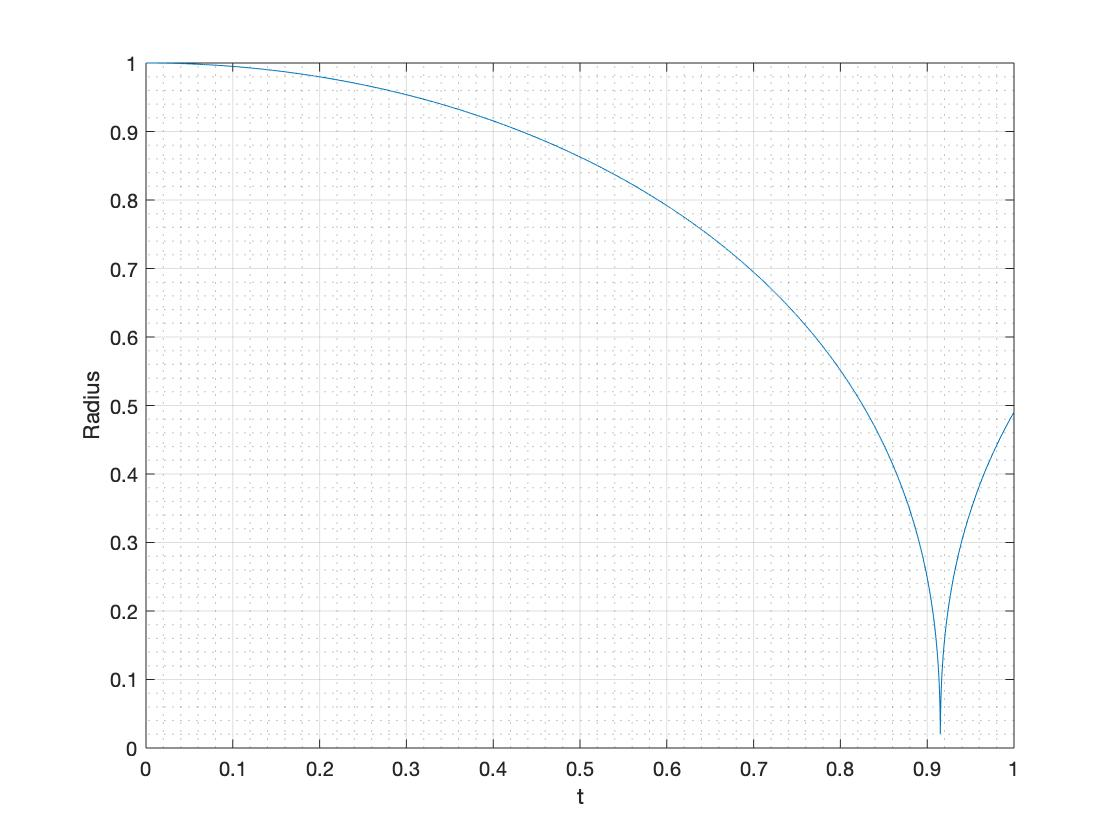
\includegraphics[width = 12cm, height = 9cm]{Q3(1).jpg}
\caption{Figure 3.1.2: Numerical solution of R against t}
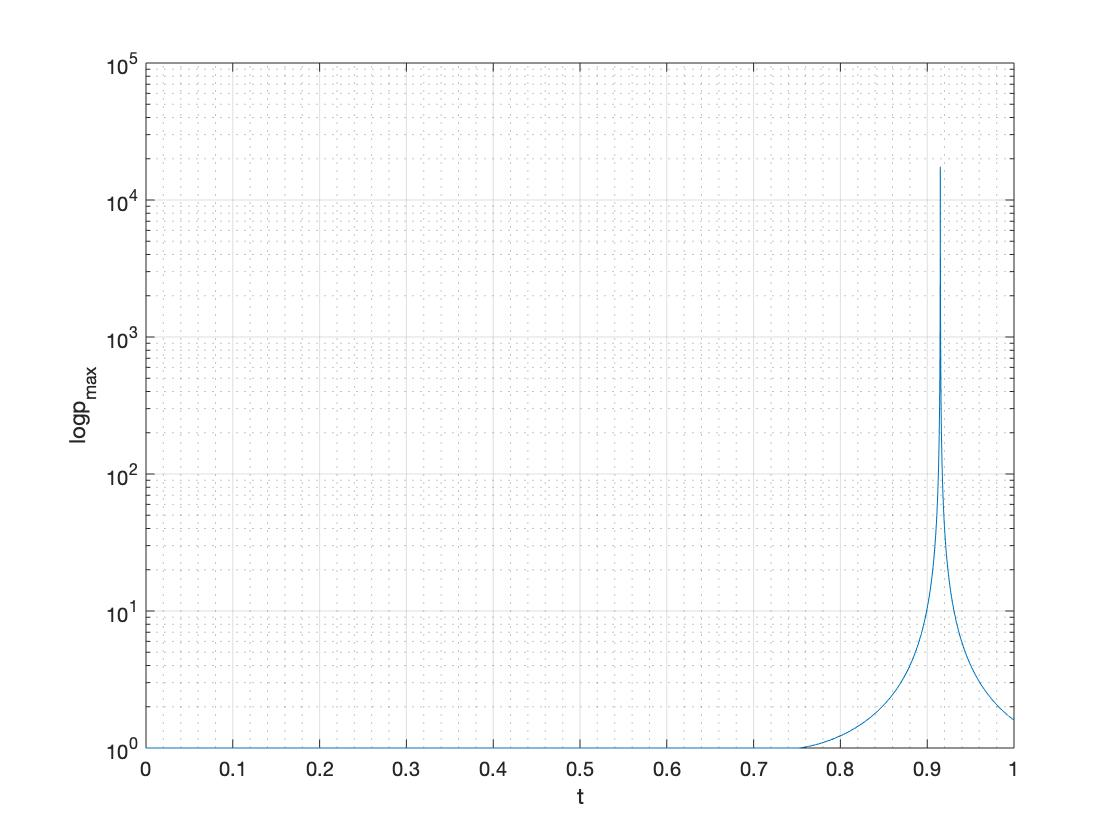
\includegraphics[width = 12cm, height = 9cm]{Q3(2).jpg}
\caption{Figure 3.1.3: Numerical solution of $p_{max}$ against t, here I use log scale in $p_{max}$}
\end{figure}
The time for collapse obtained from numerical integration is close to that by solving x numerically. Since I took 0.0001 as a start point, the starting point of x is close to 1. Also, by observing that the derivatives of x at a value close to 1 are small, the series solution can be taken as a good approximation to x when t is small. Furthermore, from previous discussion as $x \to 0$ higher order methods lose there obvious advantage over Euler method, so it is justified to apply Euler here to get the value of x near 0. Therefore, it is accurate enough to do the approximation at the start of the numerical curve and the Euler method has good accuracy near the zero point. Hence the time for collapse, which depends on the accuracy of the starting point and the zero point of the numerical curve, is reliable.
\section{With surface tension case}
\subsection{Question 4}
I chose $\lambda = 0.01, 0.1, 0.9, 100, 1000$, and include all the solutions in the same diagram as what follows. It is a representative set of values as I picked two of them $<<1$, and 1 close to 1, and two $>>1$. Therefore, we can comment on the limits when $\lambda << 1\ and\ \lambda >>1$. \newline\newline
It is evident that the time for collapse is shorter at larger surface tension. When $\lambda << 1$, the time is approximately the same as in no surface tension case. Mathematically, by continuity of the function for $\dot{x}$, and  the starting distance from the center of bubble is invariant for all cases with distinct surface tensions, we can conclude that as the time for collapse is completely dependent on $\dot{x}$ and $R(0)(i.e.\ x(0))$, when $\lambda \to 0$, $t_{c}^{[\lambda]} \to t_{c}^{[0]}$. When $\lambda >>1$, the time for collapse $\to 0$.\newline\newline
Physically, since for a larger surface tension, the pressure on the outer surface of the cavitation bubble is greater, which drives the bubble contraction quicker.
When the pressure is considerably large, the bubble collapses in an instant. When it is small, the bubble collapses in a manner approaching the time for zero surface tension case.
\begin{figure}[H]
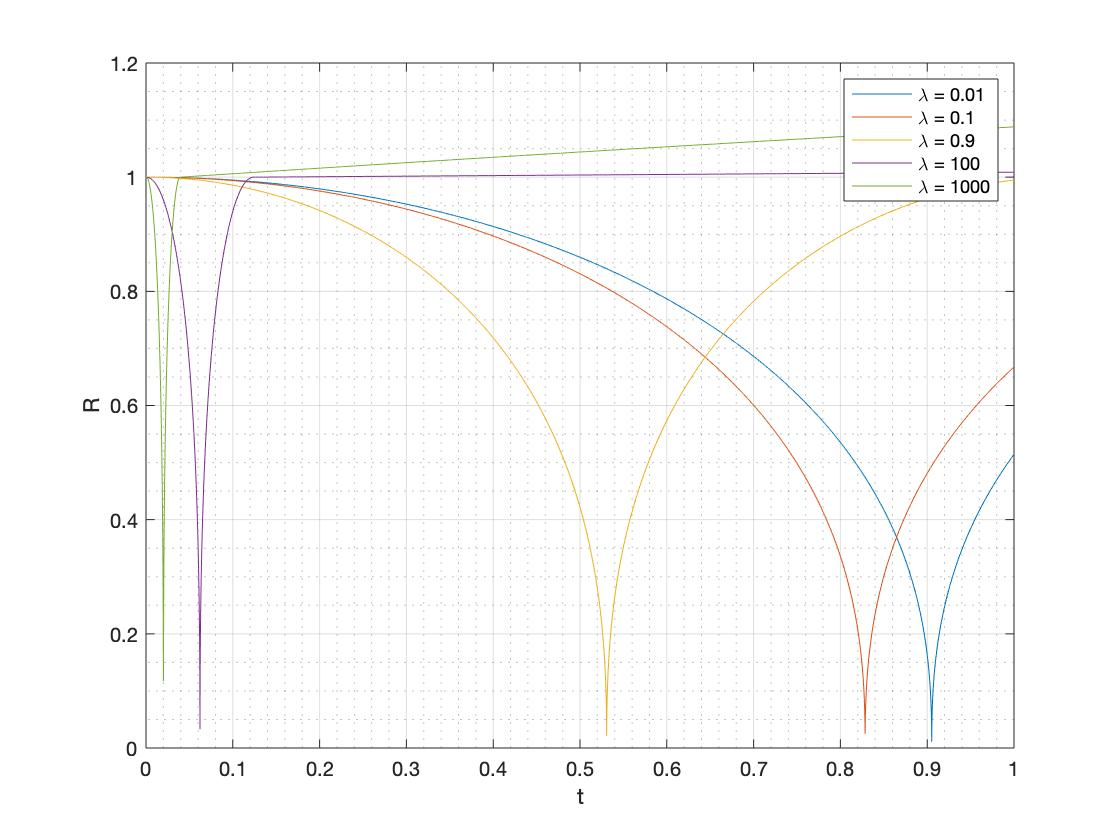
\includegraphics[width = 12cm, height = 9cm]{Q4(1).jpg}
\caption{Figure 4.1.1: Numerical solutions of R for $\lambda = 0.01, 0.1, 0.9, 100, 1000$}
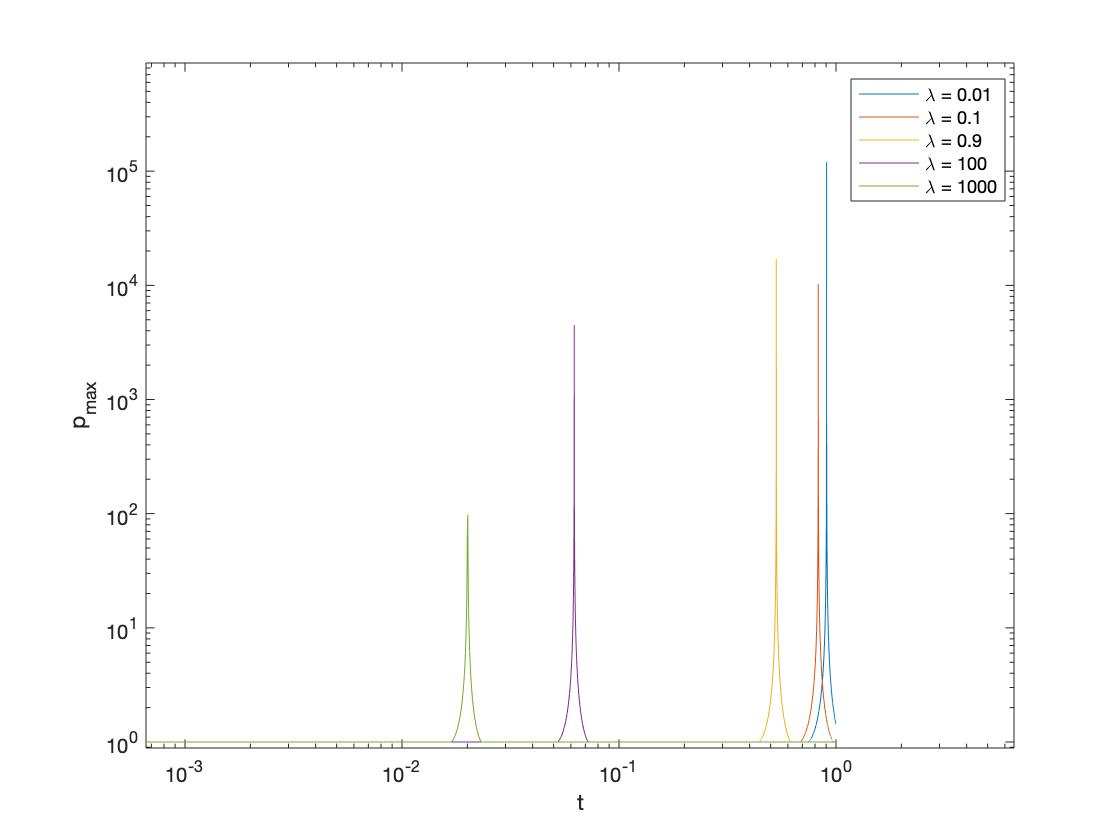
\includegraphics[width = 12cm, height = 9cm]{Q4(2).jpg}
\caption{Figure 4.1.2: Numerical solutions of $p_{max}$ for $\lambda = 0.01, 0.1, 0.9, 100, 1000$ in log scale}
\end{figure}
\subsection{Question 5}
Physical limitations:\newline
1. We can only apply it to flow with suitably low vorticity and divergence around the cavity. Actually, the surface tension is not uniform, and velocity potential is not spherically symmetric.
So we have made several simplifications. \newline
2. We have assumed that the flow extends infinitely, which is not the exact case in experimental situations. From the time-dependent Bernoulli equation, the fluid velocity might not be 0 and the time-derivative of the potential is not zero at the boundary. Thus we can only assume the flow extends infinitely when the size of bubble is extremely small.  The speed near the end of collapse (when radius is small) is overestimated as there should be another boundary condition at the actual boundary of fluid determining the pressure at a distance from the bubble. (e.g. the free surface of water)\newline
\newline\newline
Rough estimate of the initial radius as $R_{0} \simeq 1mm$, from the graph of dR/dt in Question 1, we see that the significance of pressure at infinity could be ignored (The log-log graph start to become linear) from $R/R(0) \simeq 0.7$, so below 0.7mm the physical limitations are likely to become important.
If the bubble is not empty, there is interior pressure induced by the vapour or other gas, which we assume ideal. The surface tension causes the difference between the inner and outer surfaces of the bubble, so we simply change the pressure at surface of the bubble to $p(R^{+},t) = p(R^{-},t) - 2\lambda/R$ where $p(R^{-},t)$ can be determined by volume of the bubble form the ideal gas law $pV = nRT$.
\newpage
\appendix
\section{Codes}
\subsection{Question 1}
\lstinputlisting{Q1.m}
\subsection{Question 2}
\lstinputlisting{Q2.m}
\subsection{Question 3}
\lstinputlisting{Q3.m}
\lstinputlisting{Q3_1.m}
\lstinputlisting{Q3_2.m}
\subsection{Question 4}
\lstinputlisting{Q4_1.m}
\lstinputlisting{Q4_2.m}
\end{document}